\subsection{Shape Module: Generating a Shape Descriptor}
\label{sec:architecture-shape-module}
The objective of the shape module is to combine the group descriptors $\vec{G}_g$ of an object to a single shape descriptor that can be used for the classification.
All $n_g$ group descriptors of an object are stored in $\vec{G}$ that is of size $n_g \times 6 \times 6 \times 256$.
This descriptor contains every important feature of all views and groups.
Each group descriptor $\vec{G}_g$ is fed into a fully-connected sub-network with two layers.
The first layer has $6\cdot6\cdot256$ edges per unit and 4096 units in total, while the second layer has 4069 edges per unit and 4069 output units as well.
The inputs are processed like in the fully-connected layer before.
First, each input $\vec{G}_g$ is flattened into a column-vector $\vec{g}_g$.
Then, a matrix multiplication of the inputs and the corresponding weight matrix is performed and a bias vector is added.
This result is fed into a ReLU activation function $\phi(\cdot)$ resulting in an activation for the particular layer.
In conclusion, the two fully-connected operations
\begin{subequations}
	\begin{align}
		\vec{a}^{[6]}_g &= \phi(\vec{W}^{[6]} \vec{g}_g + \vec{b}^{[6]}) \\
		\vec{a}^{[7]}_g &= \phi(\vec{W}^{[7]} \vec{a}^{[6]}_g + \vec{b}^{[7]})
	\end{align}
\end{subequations}
are performed as illustrated in \figref{fig:shape-module-group-shape}.
\begin{figure}
	\centering
	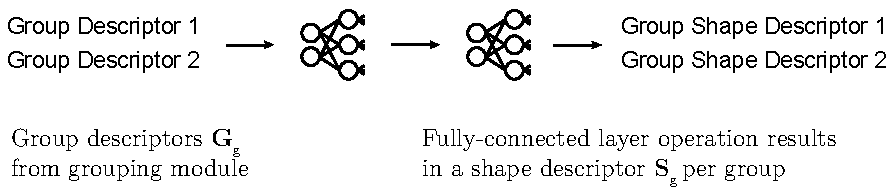
\includegraphics[]{images/shape_module_group_shape.pdf}
	\caption[Generate group shape descriptors in shape module]{Generate group shape descriptors in shape module. Each group descriptor $\vec{G}_g$ is propagated through two fully-connected layers representing layer 6 and 7 of the network. The activation of layer 7 represents the group shape descriptor $\vec{S}_g$ of each group descriptor.}
	\label{fig:shape-module-group-shape}
\end{figure}
Furthermore, both layers contain a dropout layer with a dropout probability of $0.5$.
This corresponds to the original AlexNet configuration.
Hence, the final activations of the seventh layer in the network or second dense layer, respectively, represent the shape descriptor of every group descriptor.
Those single group shape descriptor vectors of each group are and stacked along the second dimension to have a compact group shape descriptors representation $\vec{S}_{\text{groups}}$ with size $4096 \times n_g$.
Expanding this with a batch dimension yields the tensor $\bar{\vec{S}_{\text{groups}}}$ with size $Batch \times 4096 \times n_g$.

Now the group shape descriptors need to be combined for generating the final single shape descriptor of the object.
This is done by considering the corresponding group weights $\vec{w}_{\text{groups}}$ with $n_g$ elements calculated in the grouping module.
As a reminder, they are the mean of all view scores of each group, thus, an indicator for the group's discrimination.
Hence, a weighted average is calculated for considering this relation.
For this calculation the sums of the weights in inevitable.
Thus, $w_{g,\text{sum}}$ stores the sum of the group weights of an object.
The weighted average can be computed by
\begin{equation}
	\vec{s} = \frac{\vec{S}_{\text{groups}} \vec{w}_{\text{groups}}} {w_{\text{groups},\text{sum}}}
\end{equation}
where the division is performed element-wise.
The result has a shape of $4096$ and represents the final single shape descriptor.
The related assembled tensor $\bar{\vec{S}}$ has the size $Batch \times 4096$.

This representation is directly compatible with the last fully-connected layer, which is responsible for calculating the predictions of the network, thus, $\vec{s}$ is fed into it.
The number of neurons in this layer equals the number of classes where each neuron has 4096 edges.
The performed operations are identical to the ones earlier and are described by
\begin{equation}
	\vec{z}^{[8]} = \vec{W}^{[8]} \vec{s} + \vec{b}^{[8]}
\end{equation}
using the related weights and biases.
However, no activation function is applied here.
For making the predictions $\vec{z}^{[8]}$ interpretable, they are fed into a softmax layer.
This outputs a valid probability distribution $\hat{\vec{y}}$ depending on all its inputs $\vec{z}^{[8]}$.
Hence, this results in a membership probability for the network's input for each class.
The class representing the index with the largest value in $\hat{\vec{y}}$ is considered the predicted class. The functionality of the shape module is summarized in \figref{fig:shape-module-final-shape}.
\begin{figure}
	\centering
	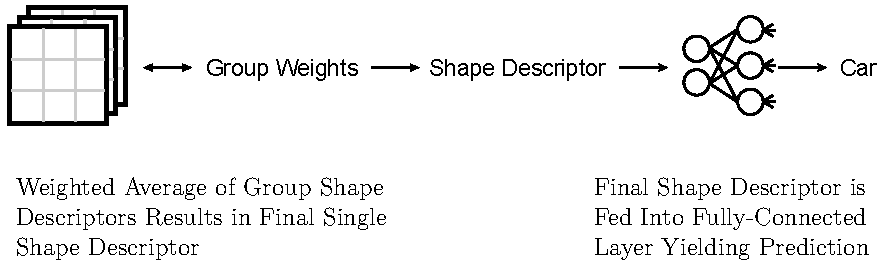
\includegraphics[]{images/shape_module_final_shape.pdf}
	\caption[Basic concept of the shape module]{Basic concept of the shape module combined with a classification. A weighted average of the group shape descriptors $\vec{S}_{\text{groups}}$ with the related group weights $w_{\text{groups}}$ is calculated yielding a single shape descriptor $\vec{s}$. It is fed into the last fully-connected layer resulting in the prediction $\hat{\vec{y}}$ of the network.}
	\label{fig:shape-module-final-shape}
\end{figure}